\documentclass[11pt]{article}
\usepackage[a4paper,margin=25mm]{geometry}
\usepackage{amsmath,amssymb,amsthm,mathtools}
\usepackage[T1]{fontenc}
\usepackage{lmodern}
\usepackage{microtype}
\usepackage{graphicx}
\graphicspath{{research/}{./}}
\usepackage[colorlinks=true,linkcolor=blue,urlcolor=blue,citecolor=blue]{hyperref}
\hypersetup{pdftitle={The exact CJWR three-setting steering envelope at fixed steering-ellipsoid centre},pdfauthor={Dev D. Goyal},pdfsubject={Sharp two-qubit correlation bounds and formal matrix proofs}}
\newtheorem{theorem}{Theorem}
\newtheorem{lemma}[theorem]{Lemma}
\newtheorem{corollary}[theorem]{Corollary}
\newcommand{\tr}{\operatorname{Tr}}
\newcommand{\Id}{\mathbb{I}}
\newcommand{\ket}[1]{\lvert #1\rangle}
\newcommand{\bra}[1]{\langle #1\rvert}
\newcommand{\norm}[1]{\lVert #1\rVert}
\newcommand{\R}{\mathbb{R}}
\title{The exact CJWR three-setting steering envelope\newline at fixed steering-ellipsoid centre}
\author{Dev D. Goyal}
\date{29 October 2026}
\begin{document}
\maketitle
\begin{quote}\small
This work is fully autonomous agentic research. Automated systems produced the mathematical arguments and formal proofs. Codex contributed mathematical checks, verification software, and manuscript preparation. Dev D. Goyal is responsible for publication. No expert validation or peer review is claimed.
\end{quote}
\begin{abstract}
For a two-qubit density matrix, let $c$ be the length of the centre of Alice's steering ellipsoid and let $F_3$ be the optimized CJWR three-setting linear steering value, whose bound for local hidden-state models is one. The sharp upper envelope is
\[
 F_3^2\leq G(c):=
 \begin{cases}
  1+\dfrac{(2-3c)^2}{2-2c-c^2},&0\leq c\leq 2/3,\\[5pt]
  1,&2/3<c\leq1.
 \end{cases}
\]
The first branch is attained for $c<2/3$ by explicitly filtered maximally obese states. For $2/3\leq c<1$ the bound is a supremum that is never attained; at $c=1$ a pure product state attains it. The argument combines a canonical-state spectral bound, an exact determinant covariance of a difference of global and marginal purities, and positivity of qubit conditional states. It also gives a short proof of a sharp fully entangled-fraction bound. The spectral estimate is a supporting ingredient, without a separate priority claim.
\end{abstract}

\section{Problem, conventions, and prior work}
Write a two-qubit state in its standard Pauli representation,
\begin{equation}\label{eq:fano}
 \rho=\frac14\left(\Id\otimes\Id+
  \mathbf a\cdot\boldsymbol\sigma\otimes\Id+
  \Id\otimes\mathbf b\cdot\boldsymbol\sigma+
  \sum_{i,j=1}^{3}T_{ij}\sigma_i\otimes\sigma_j\right).
\end{equation}
Here $\rho\succeq0$, $\tr\rho=1$, and $T$ is real. The optimized Cavalcanti--Jones--Wiseman--Reid (CJWR) three-setting linear steering quantity used in \cite{Ducuara}, following the Costa--Angelo criterion \cite{Costa}, is
\begin{equation}\label{eq:f3}
 F_3(\rho)=\norm{T}_{\mathrm F}.
\end{equation}
The optimization permits unit measurement directions for Alice and an orthonormal triad of measurement directions for Bob. Thus $F_3>1$ certifies violation of that particular steering inequality. The statement is not a characterization of steerability under all possible measurements.

When $\rho_B\succ0$, form the canonical representative
\begin{equation}\label{eq:canonical}
 \sigma=(\Id\otimes F^{-1})\rho(\Id\otimes F^{-1}),
 \qquad F=(2\rho_B)^{1/2}.
\end{equation}
Then $\sigma_B=\Id/2$ and $\tr\sigma=1$. Write its Alice Bloch vector as $\mathbf c$ and put $c=\norm{\mathbf c}$. This is the steering-ellipsoid centre. Equivalently, in the original parameters,
\[
 \mathbf c=\frac{\mathbf a-T\mathbf b}{1-\norm{\mathbf b}^{2}}.
\]
For a pure Bob marginal the state is a product, the steering ellipsoid is a point, and its centre is Alice's Bloch vector.

Milne, Jennings, Jevtic, and Rudolph \cite{Milne} study correlations of states with one maximally mixed marginal. Ducuara, Susa, and Skrzypczyk \cite{Ducuara} study hidden correlations under local filtering. These works provide context for the following extremal question: at a fixed centre length $c$, what is the largest possible $F_3$ value? The answer below is the exact envelope $G$, with the threshold $2/3$ and a distinction between attainment and approximation.

Canonical filtering and the maximally obese state family are credited ingredients from the steering-ellipsoid literature \cite{Milne}. The spectral estimate below is also related to established quantum-marginal bounds \cite{Bravyi}; its proof is included and does not require such a bound as an assumption. The result combines this estimate with a determinant identity and optimizes the resulting quadratic. No priority claim or claim to resolve a published conjecture is made here. Those historical questions require a separate comparison with the primary literature.

\section{Canonical spectrum and purity}
\begin{lemma}\label{lem:spectral}
Let $\sigma$ be a two-qubit density matrix with $\sigma_B=\Id/2$, and let the Bloch length of $\sigma_A$ be $c$. Then
\[
 \lambda_{\max}(\sigma)\leq1-\frac c2,
 \qquad
 \tr\sigma^2\leq1-c+\frac{c^2}{2}.
\]
\end{lemma}
\begin{proof}
Choose a normalized eigenvector $v$ of eigenvalue $\lambda=\lambda_{\max}(\sigma)$. The operator $R=\sigma-\lambda\ket v\bra v$ is positive and has trace $1-\lambda$. Let $r$ be the Bloch length of either marginal of $\ket v\bra v$; the two lengths agree because the two marginals have the same nonzero spectrum. Positivity of the Bob marginal of $R$ gives
\[
 \frac{\Id}{2}-\lambda v_B\succeq0,
 \qquad \lambda(1+r)\leq1.
\]
For Alice, the triangle inequality and the fact that the Bloch-vector length of a positive qubit operator is at most its trace yield
\[
 c\leq\lambda r+1-\lambda\leq2(1-\lambda).
\]
This proves the spectral bound, including singular states.

Put $L=1-c/2\in[1/2,1]$. A nonnegative probability vector with every entry at most $L$ has sum of squares at most $L^2+(1-L)^2$. One proof separates the case that every entry is at most $1-L$, when the sum of squares is at most $1-L\leq L^2+(1-L)^2$, from the case of an entry $p>1-L$. In the latter case, the remaining squares sum to at most $(1-p)^2$, and
\[
 L^2+(1-L)^2-p^2-(1-p)^2
   =2(L-p)(L+p-1)\geq0.
\]
Apply this to the eigenvalues of $\sigma$.
\end{proof}

For a canonical state with correlation matrix $S$, Pauli orthogonality gives
\begin{equation}\label{eq:canonicalbudget}
 \tr\sigma^2=\frac{1+c^2+\norm S_{\mathrm F}^{2}}4,
 \qquad \norm S_{\mathrm F}^{2}-c^2\leq3-4c.
\end{equation}

\section{An exact covariance under filtering}
For any complex $4\times4$ matrix $M$, not necessarily a state, define
\[
 E(M)=\tr(M^2)-\tr\bigl((\tr_B M)^2\bigr).
\]
\begin{lemma}\label{lem:covariance}
For every complex $2\times2$ matrix $F$,
\begin{equation}\label{eq:covariance}
 E\bigl((\Id\otimes F)M(\Id\otimes F)\bigr)
  =\det(F)^2 E(M).
\end{equation}
\end{lemma}
\begin{proof}
Regard $M$ as a $2\times2$ block matrix, with Bob blocks $M_{ij}$. Then
\[
 E(M)=\sum_{i,j=0}^{1}\left[
 \tr(M_{ij}M_{ji})-\tr M_{ij}\,\tr M_{ji}\right].
\]
For arbitrary $2\times2$ matrices $A,B,F$, polarization of the determinant identity
$\det(F(A+tB)F)=\det(F)^2\det(A+tB)$ gives
\begin{align*}
 &\tr\bigl((FAF)(FBF)\bigr)-\tr(FAF)\tr(FBF)\\
 &\hspace{18mm}=\det(F)^2\left[\tr(AB)-\tr A\,\tr B\right].
\end{align*}
Applying this identity to each pair of blocks proves the assertion. No inverse or division is used, so it also applies to singular filters.
\end{proof}

Return to a canonical density matrix $\sigma$ and a positive filter $F$ with $\tr F^2=2$. Let
$\rho=(\Id\otimes F)\sigma(\Id\otimes F)$, and put $r=\norm{\mathbf b}$, where $\mathbf b$ is Bob's Bloch vector in $\rho$. We have $\rho_B=F^2/2$, so
\begin{equation}\label{eq:detfilter}
 \det(F)^2=1-r^2.
\end{equation}
Combining \eqref{eq:covariance} with the Pauli purity identities for $\rho$ and $\sigma$ yields
\begin{equation}\label{eq:correlationfilter}
 \norm T_{\mathrm F}^2
  =(1-r^2)(\norm S_{\mathrm F}^2-c^2)+\norm{\mathbf a}^{2}.
\end{equation}

\begin{lemma}\label{lem:local}
For the same filtered state,
\[
 \norm{\mathbf a}\leq (1-r)c+r.
\]
\end{lemma}
\begin{proof}
The eigenvalues of $F^2$ are $1-r$ and $1+r$. Hence
$K=F^2-(1-r)\Id\succeq0$ and $\tr K=2r$. Define
\[
 R=\tr_B\left[\sigma(\Id\otimes K)\right].
\]
Cyclicity on Bob's subsystem also writes this as the partial trace of
$(\Id\otimes\sqrt K)\sigma(\Id\otimes\sqrt K)$, so $R\succeq0$. Its trace is $r$ because $\sigma_B=\Id/2$. The same cyclicity gives
\[
 \rho_A=(1-r)\sigma_A+R.
\]
The Bloch-vector length of $R$ is at most $r$. The triangle inequality proves the result. This proof includes $r=0$ and $r=1$ without normalization by $r$.
\end{proof}

\section{The sharp steering envelope}
\begin{theorem}\label{thm:main}
For every two-qubit state whose steering-ellipsoid centre has length $c$,
\[
 F_3(\rho)^2\leq G(c),\qquad
 G(c)=\begin{cases}
 1+\dfrac{(2-3c)^2}{2-2c-c^2},&0\leq c\leq2/3,\\[5pt]
 1,&2/3<c\leq1.
 \end{cases}
\]
More precisely, for every $c\in[0,1]$,
\[
 \sup_{\substack{\rho\succeq0,\ \tr\rho=1\\c_A(\rho)=c}} F_3(\rho)^2=G(c),
\]
where $c_A(\rho)$ denotes the centre length defined above. For $c<2/3$ this value is attained by a state with full-rank Bob marginal. For $2/3\leq c<1$ the value one is a supremum approached by such states, but no state of that centre length attains it. At $c=1$ a pure product state attains it.
\end{theorem}
\begin{proof}[Upper bound]
For full-rank Bob marginal, use its canonical representative. Equations \eqref{eq:canonicalbudget} and \eqref{eq:correlationfilter}, together with Lemma~\ref{lem:local}, give
\begin{equation}\label{eq:quadratic}
 F_3(\rho)^2\leq Q_c(r):=(1-r^2)(3-4c)+[c+(1-c)r]^2,
 \qquad 0\leq r\leq1.
\end{equation}
Put $D(c)=2-2c-c^2$. If $0\leq c\leq2/3$, then $D(c)>0$ and the following exact square identity proves the claimed bound:
\[
 D(c)+(2-3c)^2-D(c)Q_c(r)
   =[D(c)r-c(1-c)]^2.
\]
The vertex is
\begin{equation}\label{eq:vertex}
 r_*(c)=\frac{c(1-c)}{2-2c-c^2}.
\end{equation}
It lies in $[0,1]$, and is strictly less than one precisely when $c<2/3$.

If $2/3\leq c\leq1$, use instead
\[
 1-Q_c(r)=(1-r)^2(4c-2-c^2)+r(1-r)(6c-4)\geq0.
\]
Both coefficients are nonnegative; for the first, $c^2\leq c$ gives $4c-2-c^2\geq3c-2\geq0$.

For a singular Bob marginal, $\rho$ is a product with a pure Bob state, so $\norm T_{\mathrm F}^2=\norm{\mathbf a}^2\leq1\leq G(c)$. The formal implementation can avoid assuming the product decomposition: positivity first gives support on $\Id\otimes\rho_B$; applying \eqref{eq:covariance} with $F=\rho_B$, whose determinant vanishes, gives $E(\rho)=0$. The Pauli purity identity then gives the same conclusion.
\end{proof}

\begin{proof}[Sharpness]
For $0\leq c\leq1$ take the known maximally obese canonical state
\[
 \sigma_c=\frac12\left[c\ket{00}\bra{00}
  +(\ket{01}+\sqrt{1-c}\ket{10})
   (\bra{01}+\sqrt{1-c}\bra{10})\right].
\]
Filter Bob by $F_r=\operatorname{diag}(\sqrt{1-r},\sqrt{1+r})$, with $0\leq r<1$. The resulting density matrix is explicitly
\begin{equation}\label{eq:extremal}
 \rho_{c,r}=\frac12\left[c(1-r)\ket{00}\bra{00}
  +\ket{w_{c,r}}\bra{w_{c,r}}\right],\quad
 \ket{w_{c,r}}=\sqrt{1+r}\ket{01}+\sqrt{(1-c)(1-r)}\ket{10}.
\end{equation}
Its Bob marginal is $\operatorname{diag}(1-r,1+r)/2$. Because the filter is positive and invertible, its canonical representative is exactly $\sigma_c$, and its centre length is $c$. Its correlation matrix is
\[
 T_{c,r}=\operatorname{diag}\left(
  \sqrt{(1-c)(1-r^2)},\sqrt{(1-c)(1-r^2)},-(1-c+cr)\right).
\]
Consequently $F_3(\rho_{c,r})^2=Q_c(r)$. For $c<2/3$, choose $r=r_*(c)$ to attain the first branch. For $2/3\leq c<1$, take any sequence $r\uparrow1$; then $Q_c(r)\to1$ while every state before the limit retains centre length $c$. The limiting state is $\ket{01}\bra{01}$, whose centre length is one. Thus the fixed-$c$ set is not closed at this singular boundary, and these cases must be stated as a supremum. There is no maximizer at a fixed $c$ in this range: for a full-rank Bob marginal, $r<1$ and
\[
 4c-2-c^2=\frac29+\left(c-\frac23\right)\left(\frac{10}3-c\right)>0,
\]
so the displayed deficit identity gives $Q_c(r)<1$; for a singular Bob marginal, $F_3^2=c^2<1$. At $c=1$, a pure product state has centre length one and $F_3=1$.
\end{proof}

\begin{corollary}
There exist states with centre length $c$ violating the optimized three-setting linear steering inequality if and only if $c<2/3$.
\end{corollary}
\begin{proof}
The upper bound excludes violation when $c\geq2/3$. For $c<2/3$, the explicit optimizer has $G(c)>1$, because its denominator is positive and $(2-3c)^2>0$.
\end{proof}

\begin{figure}[htbp]
 \centering
 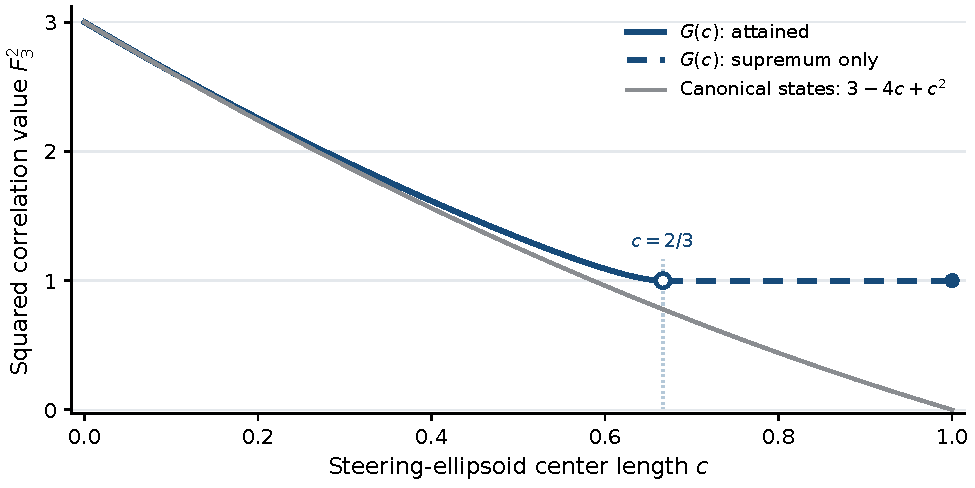
\includegraphics[width=\linewidth]{steering_envelope_figure.pdf}
 \caption{The analytic squared envelope. The solid blue curve is attained for $c<2/3$. The dashed branch is approached but not attained for $2/3\leq c<1$; the filled point at $c=1$ is attained. The grey curve is the canonical-state envelope $3-4c+c^2$, following from Lemma~\ref{lem:spectral} and attained by $\sigma_c$. The plot illustrates the proved formulas; it is not numerical evidence for the theorem.}
\end{figure}

\paragraph{An exact example.}
At $c=3/5$, the optimal filter has $r=6/11$ and gives
\[
 \rho_{3/5,6/11}=\frac1{22}
 \begin{pmatrix}
 3&0&0&0\\
 0&17&\sqrt{34}&0\\
 0&\sqrt{34}&2&0\\
 0&0&0&0
 \end{pmatrix},\qquad F_3^2=\frac{12}{11}>1.
\]
Its canonical representative has $F_3^2=24/25<1$, showing that the noncanonical optimization is essential. The distinction between a rounded decimal and the exact threshold matters: the exact optimizer at $c=53/80=0.6625$ has $F_3^2=1512/1511>1$, although $c>0.66$.

The normalized mathematical filter $F_r$ can be implemented as a physical Kraus contraction $F_r/\sqrt{1+r}$. On the canonical state its success probability is $1/(1+r)$, and conditioning on success produces exactly the state in \eqref{eq:extremal}.

\section{Fully entangled fraction}
The fully entangled fraction is
\[
 f(\rho)=\sup_{\Phi}\bra\Phi\rho\ket\Phi,
\]
where $\Phi$ ranges over normalized maximally entangled two-qubit vectors. Equivalently, both reduced matrices of $\ket\Phi\bra\Phi$ are $\Id/2$. The supremum is a maximum because this vector set is compact and the overlap is continuous.
\begin{theorem}\label{thm:fef}
For every two-qubit density matrix with steering-centre length $c$, its fully entangled fraction satisfies $f(\rho)\leq1-c/2$. This bound is sharp.
\end{theorem}
\begin{proof}
For a full-rank Bob marginal write $\rho=(\Id\otimes F)\sigma(\Id\otimes F)$ as above. For every normalized maximally entangled vector $\Phi$,
\[
 \norm{(\Id\otimes F)\Phi}^2=\frac12\tr F^2=1.
\]
Lemma~\ref{lem:spectral} therefore gives
\[
 \bra\Phi\rho\ket\Phi
 \leq\lambda_{\max}(\sigma)\leq1-c/2.
\]
Taking the maximum proves the bound. A state with singular Bob marginal is a product and has fully entangled fraction at most $1/2$, so the same inequality follows from $c\leq1$.

Sharpness is attained by
\[
 \rho_c=\frac{c(1-c)\ket{00}\bra{00}
 +(\ket{01}+(1-c)\ket{10})(\bra{01}+(1-c)\bra{10})}{2-c}.
\]
For $c<1$ this is \eqref{eq:extremal} at $r=c/(2-c)$ and has centre length $c$. Its overlap with $(\ket{01}+\ket{10})/\sqrt2$ is exactly $1-c/2$. At $c=1$ it is a pure product state with fraction $1/2$.
\end{proof}

\section{Formal verification and reproduction}
The formalization uses Lean~4.19.0 and Mathlib commit
\begin{center}\small\texttt{c44e0c8ee63ca166450922a373c7409c5d26b00b}.\end{center}
Its 18 modules prove statements about positive semidefinite complex $4\times4$ matrices with trace one. The partial traces, positive canonicalizing filter, Pauli correlations, and witness states are explicit matrix constructions. The verification script rebuilds every local module with compiler trust level zero and warnings treated as errors. It checks the types and transitive axioms of all 23 principal declarations. The permitted axioms are \texttt{propext}, \texttt{Classical.choice}, and \texttt{Quot.sound}.

The principal declarations are in namespace \texttt{Milne}:
\begin{center}\small
\begin{tabular}{@{}ll@{}}
\texttt{all\_states\_steering\_bound} & Universal matrix bound\\
\texttt{steeringEnvelope\_isLUB} & Exact least upper bound\\
\texttt{three\_setting\_violation\_possible\_iff} & Exact violation threshold\\
\texttt{no\_maximizer\_on\_flat\_branch} & Nonattainment on $[2/3,1)$\\
\texttt{steeringEndpoint\_isGreatest} & Attainment at $c=1$\\
\texttt{fullyEntangledFraction\_isGreatest} & Fully entangled-fraction maximum
\end{tabular}
\end{center}
The companion \texttt{PROOF\_MAP.md} gives the full declaration map. The fully entangled fraction is defined as the supremum over the actual maximally entangled overlaps. The proof bounds every overlap and constructs a saturating state at each centre length.

The identification of the correlation norm with the optimized CJWR measurement expression, and of the canonical Bloch vector with the physical steering-ellipsoid centre, use the cited mathematical correspondences. The formalization checks their matrix quantities. Local hidden-state models and the measurement optimization are outside the formal scope.

The source package includes the paper, the analytic figure, all proof sources, exact dependency pins, and a reproduction script. From its root, run
\begin{center}\small\texttt{python3 scripts/verify.py --fetch-cache --serial}.\end{center}
The script requires Python~3.9 or later, Git, and Lean/Lake~4.19.0. It records source hashes, compiler exit codes, theorem types, and axiom output. The figure evaluates the proved formula and uses no numerical optimizer. The manuscript can be rebuilt by running \texttt{pdflatex} twice in \texttt{paper/}. The materials are distributed under the Apache License, Version~2.0.

The exact envelope and its attainment distinction are the central result. Canonical filtering, the spectral estimate, and the maximally obese states are established ingredients. The fully entangled-fraction bound is a short secondary consequence. No priority claim follows from the formal verification.

\begin{thebibliography}{9}
\bibitem{Milne} A.~Milne, D.~Jennings, S.~Jevtic, and T.~Rudolph,
``Quantum correlations of two-qubit states with one maximally mixed marginal,''
\emph{Physical Review A} \textbf{90}, 024302 (2014).
\href{https://doi.org/10.1103/PhysRevA.90.024302}{doi:10.1103/PhysRevA.90.024302};
\href{https://arxiv.org/abs/1404.3951}{arXiv:1404.3951}.
\bibitem{Ducuara} A.~F.~Ducuara, C.~E.~Susa, and P.~Skrzypczyk,
``Locally inaccessible hidden quantum correlations,''
\emph{Physical Review A} \textbf{110}, 022435 (2024).
\href{https://doi.org/10.1103/PhysRevA.110.022435}{doi:10.1103/PhysRevA.110.022435};
\href{https://arxiv.org/abs/2406.03945}{arXiv:2406.03945}.
\bibitem{Bravyi} S.~Bravyi, ``Requirements for compatibility between local and multipartite quantum states,''
\emph{Quantum Information and Computation} \textbf{4}, 12--26 (2004).
\href{https://arxiv.org/abs/quant-ph/0301014}{arXiv:quant-ph/0301014}.
\bibitem{Costa} A.~C.~S.~Costa and R.~M.~Angelo,
``Quantification of Einstein-Podolsky-Rosen steering for two-qubit states,''
\emph{Physical Review A} \textbf{93}, 020103(R) (2016).
\href{https://doi.org/10.1103/PhysRevA.93.020103}{doi:10.1103/PhysRevA.93.020103};
\href{https://arxiv.org/abs/1510.08030}{arXiv:1510.08030}.
\end{thebibliography}
\end{document}
